\newcommand{\BolognaBackgroundPic}{%
  \put(0,0){%
    \parbox[b][\paperheight]{\paperwidth}{%
      % Original picture:
      % https://commons.wikimedia.org/wiki/File:Bologna-SanPetronioPiazzaMaggiore1.jpg
      % Distributed by the author under the GNU FDL v1.2 and Creative Commons Attribution-Share Alike 3.0
      \vfill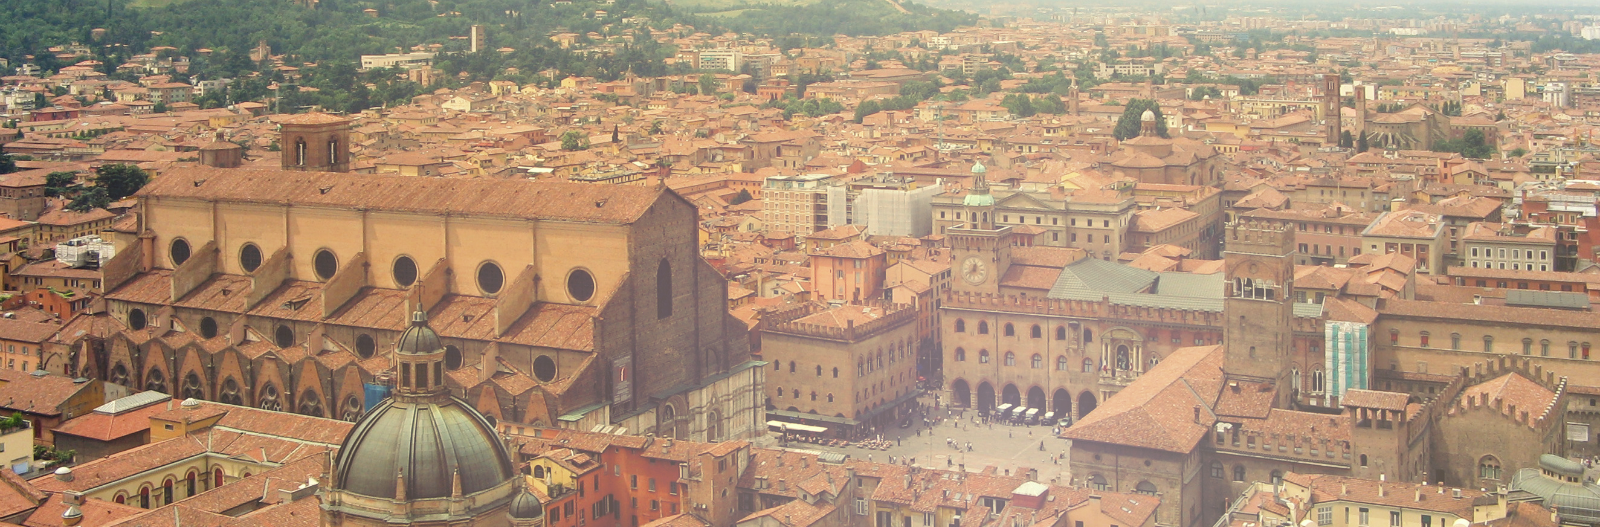
\includegraphics[width=\paperwidth,height=\paperheight,keepaspectratio]{./figures/bologna_strip.png}
    }
  }
}

\newgeometry{top=2.4cm,bottom=2.4cm,left=2.4cm,right=2.4cm}
\makeatletter

\begin{titlepage}
  \AddToShipoutPicture*{\BolognaBackgroundPic}
  
  \begin{center}
      \vspace*{1em}
      
\includegraphics[height=6em,keepaspectratio]{./figures/unibo_logo.png}\\
      %{\scshape\small Electric, Electronic and Information Engineering Department}\\[2em]
      \vspace{10em}
      {\sffamily\Huge \@title}\\[2em]
      {\sffamily Technical Report \TechReportNumber}\\[4em]
      {\sffamily\Large \@author}\\[2em]
      {\sffamily \@date}
      \vfill
      \begin{tikzpicture}[overlay, remember picture]
        \fill[black,opacity=0.5] (-12,-0.4) rectangle (12,-2.4);
        \node[color=white] at (-5,-1.4) {\sffamily {\Huge OR-Unibo}~~~Operational Research Group};
        % Twitter logo obtained from http://about.twitter.com/
        \node at (7,-1.4) {
\includegraphics[height=1.5em,keepaspectratio]{./figures/twitter_logo.png}};
        \node[color=white] at (8.75,-1.5) {\sffamily @OR\_Unibo};
      \end{tikzpicture}
  \end{center}
\end{titlepage}

\makeatother
\restoregeometry